\label{sub:SpecO}


Our assertions are  %\AssertLang, 
 standard  (\eg properties of the values of expressions,  connectives, quantification \etc),    about protection (\ie ${\protectedFrom{{\re}} {{\re}}} $ and 
$ {\inside {{\re}}} $), and about adherence to Specifications.


% \emph{object capability}. 
% Standard assertions assert properties of the values of fields, implication, quantification etc, as well as ghost fields  which represent user-defined predicates. 
%Object capability assertions express restrictions of  objects' \fbox{eventual authority} on other objects.

\begin{definition}
\label{def:assert:syntax}
%Expressions, $\re$, 
%Assertions, $A$,  are defined as follows:
%
%\label{f:chainmail-syntax}
%$
%\begin{syntax}
%\syntaxElement{A\ \ }{}
%		{
%		\syntaxline
%				{{\re}}
%				{{\re} : C}
%				{\external{{\re}}}
% 				{\protectedFrom{{\re}} {{\re}}} 
%				 {\inside {{\re}}} 
%				 {\obeys {\re} {S}}
%				 {\neg A}
%				{A\ \wedge\ A}
%				{\all{x:C}{A}}				
%		\endsyntaxline
%		}
%\endSyntaxElement\\
%\end{syntax}
%$

We   define concrete assertions $\co {A}$, assertions which contain no $\textbf{obeys}$ clauses $\no{A}$, and well-formed assertions $\wf {A}$, as follows (where $S$ stands for a specification identifier):

$
\begin{syntax}
\syntaxElement{\co A}{}
		{
		\syntaxline
				{{\re}}
				{{\re} : C}
				{\external{{\re}}}
 				{\protectedFrom{{\re}} {{\re}}} 
				 {\inside {{\re}}} 
				  {\neg \co A}
				{\co A\ \wedge\ \co A}			
		\endsyntaxline
		}
\endSyntaxElement
 \\
\syntaxElement{\no A}{}
		{
		\syntaxline
				{{\re}}
				{{\re} : C}
				{\external{{\re}}}
 				{\protectedFrom{{\re}} {{\re}}} 
				 {\inside {{\re}}} 
				  {\neg \no A}
				{\no A\ \wedge\ \no A}
								{\all{x:C}{\no A}}				
		\endsyntaxline
		}
\endSyntaxElement
\\
\syntaxElement{\wf A  }{}
		{
		\syntaxline
				{{\re}}
				{{\re} : C}
				{\external{{\re}}}
 				{\protectedFrom{{\re}} {{\re}}} 
				 {\inside {{\re}}} 
				{\neg \no A}
				{\wf A\ \wedge\ \wf A \strut \  \ \  \ }
				{\all{x:C}{\wf A} }	
				 {\obeys {\re} {S}}				 			
		\endsyntaxline
		}
\endSyntaxElement
\end{syntax}
$

 
\end{definition}

Concrete assertions, $\co A$ will be used when modules give meaning to abstract predicates, and obeys-free assertions $\no A$ are used in order to ensure that $\textbf{obeys}$ clauses do not appear in negative positions in our assertions $\wf A$.
 
%\label{def:chainmail-semantics-all}
%\label{dup:def:chainmail-semantics}
%\noindent
 Satisfaction  of  obeys-free assertions, $\no A$ by a module and a state is expressed  through \ $\satisfiesA{M}{\sigma}{{\no A}}$ \  and defined by cases on the shape of $\no A$, in definitions \ref{def:chainmail-semantics}.


\begin{definition}[Satisfaction 
of Assertions -- first part] 
\label{def:chainmail-semantics}
\label{def:chainmail-protection-from}
\label{sect:semantics:assert:prtFrom}
 \label{def:chainmail-protection}
 We define satisfaction of obeys=free assertions $\no A$ by a % program 
state $\sigma$ with 
 module $M$ as:
\begin{enumerate}
\item
\label{cExpr}
$\satisfiesA{M}{\sigma}{{\re}}\ \ \ \triangleq \ \ \   \eval{M}{\sigma}{{\re}}{\true}$
\item
\label{cClass}
$\satisfiesA{M}{\sigma}{{{\re}} : C}\ \ \ \triangleq \ \ \   \eval{M}{\sigma}{{\re}}{\alpha}\   \wedge \ \class{\alpha} {\sigma}= C$
\item
\label{cExternal}
$\satisfiesA{M}{\sigma}{\external{{\re}}} \ \ \ \triangleq \ \ \  \exists C.[\ \satisfiesA{M}{\sigma}{{{\re}} : C} \ \wedge \ C \notin M \ ]$
 \item
 \label{cProtected}
$\satisfiesA{M}{\sigma}{\protectedFrom{{\re}} {{\re_{o}}}}$ $\ \  \triangleq\ \ $
$\exists \alpha, \alpha_{o}. [\  \ \  \eval{M}{\sigma}{{\re}}{\alpha}\ \ \ \wedge\ $

  \begin{enumerate}
 \item
$\alpha\neq \alpha_0$,
 \item
$\forall \alpha'.\forall f.[\ \alpha' \in {\Relevant {\alpha_o} {\sigma}} \wedge\   \satisfiesA{M}{\sigma}{\external {\alpha'}} 
\ \ \Longrightarrow \ \  
  \interpret {\sigma} {\alpha'.f} \neq \alpha     \ ] $.
\end{enumerate}

$  \strut \hspace{4cm} ] $.
 \item
 \label{sect:semantics:assert:prt}
$\satisfiesA{M}{\sigma}{\protectedFrom{{\re}} {{\re_{o}}}}$ $\ \  \triangleq\ \ $
$\exists \alpha, \alpha_{o}. [\  \  \eval{M}{\sigma}{{\re}}{\alpha}\ \wedge\ \eval{M}{\sigma}{{\re_0}}{\alpha_0} \  \wedge$  % 

\begin{enumerate}
\item
 $\satisfiesA{M}{\sigma}{\extThis}\ \ \Longrightarrow\ \ \forall x\!\in\! \sigma.\ \satisfiesA{M}{\sigma}{x\neq \alpha}$,
 \item
$\forall \alpha'.\forall f.[\ \alpha' \in {\LRelevantO {\sigma}} \wedge\   \satisfiesA{M}{\sigma}{\external {\alpha'}} 
\ \ \Longrightarrow \ \  
  \interpret {\sigma} {\alpha'.f} \neq \alpha     \ ]$ 
  \end{enumerate} 
$  \strut \hspace{4cm} ] $.

  \item
$\satisfiesA{M}{\sigma}{\neg \no A}\ \ \ \triangleq \ \ \   {M},{\sigma}\not\models{\no A}$
\item
$\satisfiesA{M}{\sigma}{\no A_1\ \wedge\ \no A_2}\ \ \ \triangleq \ \ \   \satisfiesA{M}{\sigma}{\no A_1} \   \wedge \ \satisfiesA{M}{\sigma}{\no A_2}$
\item
\label{quant1}
$\satisfiesA{M}{\sigma}{\all{x:C}{\no A}} \ \ \ \triangleq \ \ \   
\forall \alpha.[\   \satisfiesA {M}{\sigma} {\alpha:C}  \ \Longrightarrow   \ \satisfiesA{M}{\sigma} {\no A[\alpha/x]} \ ] $
\end{enumerate}

 \end{definition} 
% 
% We illustrate ``protected'' and ``protected from'' in Fig.  \ref{fig:ProtectedBoth} in \S \ref{s:outline}.
%% that appendex commented out from all version of main.tex
%   and    Fig.  \ref{fig:ProtectedFrom} in App. \ref{appendix:assertions}.
%%
%In general,  $\protectedFrom{{\alpha}} {{\alpha_{o}}}$ ensures that $\alpha_o$ will get access to $\alpha$ only if another object 
% % an internal object 
% grants that access.
%Similarly, $\inside \alpha$ ensures that during execution of the current method, no external object will get direct access to $\alpha$ unless some internal object grants that access\footnote{This is in line with the motto "only connectivity begets connectivity" from \cite{MillerPhD}.}.
%Thus, protection together with protection preservation  (\ie no internal object gives access) guarantee
%%are sufficient but not necessary conditions for 
%lack of eventual external access.  
%
% 
%\footnoteSD{JAMES' comment: If is possible that ``we'' do not know the complete heap (eg we only know about the green stuff.) how do we know whether an object is protected. The answer is that we do not know that it is protected, but we do know that our code guarnartees poreservation of protectedness.
%}  
% 
% \subsubsection*{Discussion} 
%Lack of  eventual 
%direct access is a central concept in the verification of code with calls to and callbacks  from untrusted code.
%% ARGHHH a joke citatiion? \cite{praiseYou}.   
%%Unmediated access is essentially \citet{MillerPhD}'s permission: that we have a ``first
%%class'' reference to the capability; that we can call any 
%%method in the capability's public interface; that we can
%%store or save or present the capability to any other
%%object to which we've been introduced
%%%\footnote{``nobody can ever be introduced in a ball-room''}
%It has already been over-approximated in several different ways, \eg
%2nd-class \cite{rompf-second-class-oopsla2016,rompf-dont-pop-second-class-ecoop2022}
%or borrowed (``2nd-hand'') references
%\cite{boyland-promises-icse1998,boyland-aliasburying-spe2001},
% textual modules \cite{OOPSLA22},
%information flow \cite{ddd}, runtime
%checks \cite{secure-io-fstar-popl2024},
%abstract data type exports \cite{vmsl-pldi2023},
%  separation-based invariants 
%Iris \cite{iris-wasm-pldi2023,cerise-jacm2024},
%-- more in  \S~\ref{sect:related}.
%In general, protection is applicable in more situations (i.e.\ is less
%restrictive) than most of these approaches,
% although more restrictive than the ideal ``lack of eventual access''. 
%\footnoteSD{ HER WHAT IT USED TO SAY: the contrapositive ideal that lack of eventual access ensures
%lack of effect. Note that ``cannot get direct access'' does not generally imply ``is protected''. 
%}
%
%
%
%
%
%\noindent
%\begin{flushleft}
%\begin{tabular}{@{}lr@{}}
%  \begin{minipage}{.85\textwidth}
%   {An alternative definition might consider $\alpha$ as protected from $\alpha_o$, 
%if   any path from $\alpha_o$ to $\alpha$ goes through at least one internal object.
%With this definition, $o_4$ would be protected from $o_1$ in the heap shown here.
%However,  $o_1$ can make a call to $o_2$, and  this call could  return $o_3$. 
%Once $o_1$ has direct access to $o_3$, it can also get direct access to $o_4$. 
%The example justifies our current definition.  
%}
%\end{minipage}
%& 
%\begin{minipage}{.18\textwidth}
%\resizebox{2cm}{!}{
%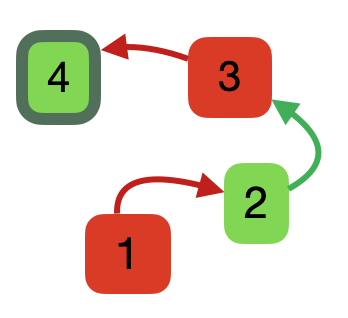
\includegraphics[width=\linewidth]{diagrams/altDef.png}
%} 
%\end{minipage}
%\end{tabular}
%\end{flushleft}
%
%
%%Protection --- \sdN{objects to which external objects may not get %which objects can get 
%%unmediated access} % to which other objects 
%%---  is  a crucial concept: It enables
%%the verification code in the open world, % even in the presence of
%%with calls to and callbacks 
%%from untrusted code.
%%% ARGHHH a joke citatiion? \cite{praiseYou}.   
%%Unmediated access is essentially \citet{MillerPhD}'s permission: that we have a ``first
%%class'' reference to the capability; that we can call any 
%%method in the capability's public interface; that we can
%%store or save or present the capability to any other
%%object to which we've been introduced
%%%\footnote{``nobody can ever be introduced in a ball-room''}
%%(compare
%%2nd-class \cite{rompf-second-class-oopsla2016,rompf-dont-pop-second-class-ecoop2022}
%%or borrowed (``2nd-hand'') references
%%\cite{boyland-promises-icse1998,boyland-aliasburying-spe2001}
%%which are restricted in some way),
%%without reference to some owning class or defining module.
%%We discuss alternative designs,
%%ranging from overly simplistic textual modules \cite{OOPSLA22},
%%information flow \cite{ddd}, runtime
%%checks \cite{secure-io-fstar-popl2024},
%%abstract data type exports \cite{vmsl-pldi2023},
%%to automated separation-based invariants in
%%Iris \cite{iris-wasm-pldi2023,cerise-jacm2024},
%%in section~\ref{sect:related}.
%%In general, protection is applicable in more situations (i.e.\ is less
%%restrictive) than most of these approaches,
%% \sdN{although more restrictive than the ideal "lack of eventual permission"}. 
%%\footnoteSD{ HER WHAT IT USED TO SAY:
%%the contrapositive ideal that lack of eventual permission ensures
%%lack of effect. Note that ``cannot get direct access'' does not generally imply ``is
%%protected''


 
